\section{Requirement 3: Test cases for ONE physical product}

\subsection{Thông tin thiết bị}
- \textbf{Loại thiết bị: } Quạt điện đứng

- \textbf{Hãng sản xuất: } JIO

- \textbf{Mẫu mã: } BHL - 086

- \textbf{Năm sản xuất: } Khoảng 2010

- \textbf{Số seri: } unknown

\subsection{Hình ảnh thiết bị và thông tin sinh viên đính kèm}
\begin{figure}[H]
    \centering
    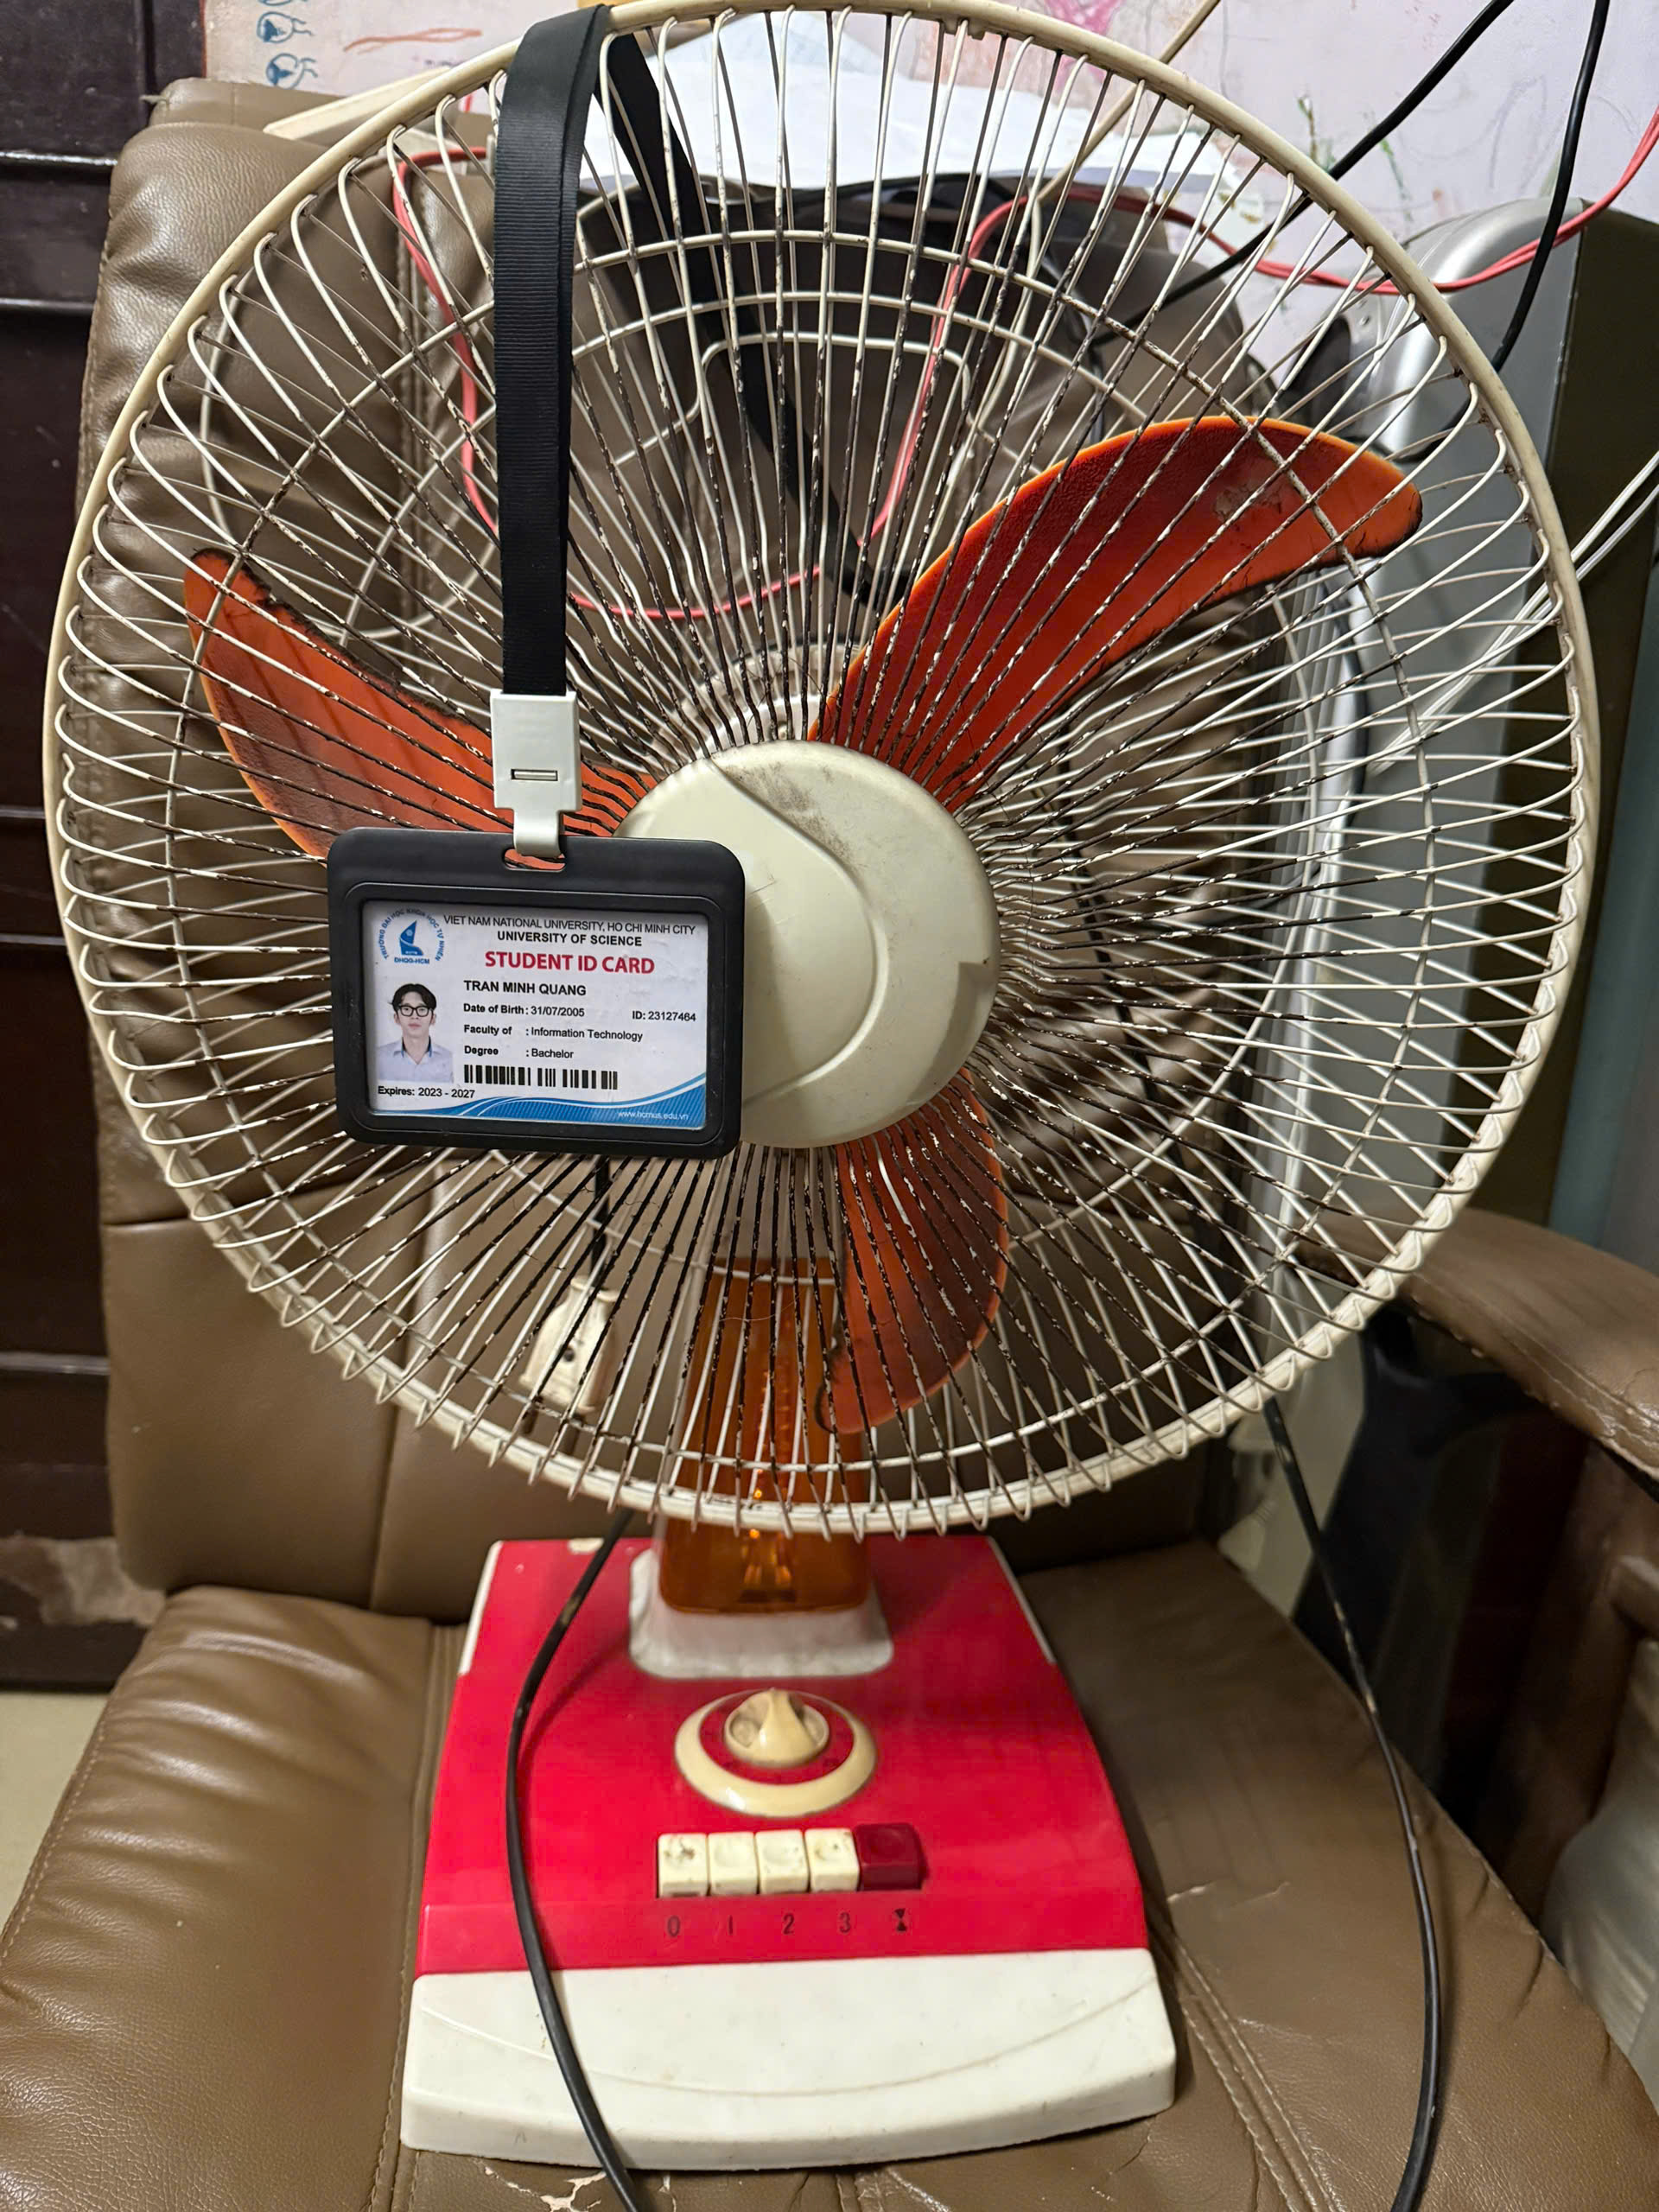
\includegraphics[width=0.5\textwidth]{System_with_studentID/fan_and_studentID.jpg}
    \caption{Hình ảnh quạt điện cùng với bảng thông tin sinh viên.}
    \label{fig:fan}
\end{figure}

\subsection{Test cases}

\begingroup
\scriptsize
\setlength{\LTleft}{0pt}
\setlength{\LTright}{0pt}

\begin{longtblr}[
  caption = {Bảng Test Cases -- Quạt điện đứng JIO BHL-086},
  label = {tab:testcases},
]{
  colspec = {|Q[c,m,0.06\linewidth]|Q[l,m,0.14\linewidth]|Q[l,m,0.14\linewidth]|Q[l,m,0.20\linewidth]|Q[l,m,0.20\linewidth]|Q[c,m,0.09\linewidth]|Q[c,m,0.07\linewidth]|},
  rowhead = 1,
  row{1} = {font=\bfseries, bg=blue!20, c, m},
  row{even} = {bg=gray!8},
  hlines,
  vlines,
  cells = {font=\scriptsize},
}
ID & Mục tiêu & Đầu vào / Điều kiện & Các bước thực hiện & Kết quả mong đợi & Thực tế & Verdict \\
TC-01
& Kiểm tra chức năng khởi động quạt.
& Quạt được cắm nguồn điện 220V, đang ở trạng thái Tắt.
& 1. Bấm nút nguồn hoặc nút chọn mức gió thấp nhất (Mức 1).
& Quạt bắt đầu hoạt động, cánh quạt quay đều, không có tiếng kêu lạ.
& Quạt hoạt động ổn định.
& PASSED \\
TC-02
& Kiểm tra chức năng tắt quạt.
& Quạt đang hoạt động ở mức gió bất kỳ.
& 1. Bấm nút Tắt (Off).
& Quạt ngắt điện ngay lập tức, cánh quạt giảm tốc rồi dừng hẳn.
& Quạt dừng hoàn toàn, không còn quay.
& PASSED \\
TC-03
& Kiểm tra chức năng tăng mức gió (Mức trung bình).
& Quạt đang chạy ở mức gió 1 (Thấp).
& 1. Bấm nút chọn mức gió 2 (Trung bình).
& Tốc độ vòng quay của cánh quạt tăng lên rõ rệt, luồng gió mạnh hơn.
& Quạt hoạt động ổn định.
& PASSED \\
TC-04
& Kiểm tra chức năng tăng mức gió (Mức cao nhất).
& Quạt đang chạy ở mức gió 2 (Trung bình).
& 1. Bấm nút chọn mức gió 3 (Cao nhất).
& Tốc độ cánh quạt quay ở mức tối đa, động cơ không có mùi khét.
& Quạt hoạt động ổn định.
& PASSED \\
TC-05
& Kiểm tra chuyển đổi mức gió từ Cao về Thấp.
& Quạt đang chạy ở mức gió 3 (Cao nhất).
& 1. Bấm trực tiếp nút chọn mức gió 1 (Thấp).
& Quạt nhận tín hiệu ngay, tốc độ vòng quay giảm dần xuống mức thấp.
& Tốc độ quay giảm rõ rệt không có dấu hiệu chập chờn.
& PASSED \\
TC-06
& Kiểm tra chức năng xoay ngang (Tuốc năng).
& Quạt đang chạy, lồng quạt đứng yên.
& 1. Nhấn (hoặc gạt) nút bấm phía sau motor quạt.
& Bầu quạt bắt đầu tự động xoay chuyển hướng gió sang trái và phải đều đặn.
& Quạt hoạt động ổn định.
& PASSED \\
TC-07
& Kiểm tra chức năng dừng xoay ngang.
& Quạt đang chạy và đang xoay ngang đều đặn.
& 1. Rút (hoặc gạt ngược lại) nút bấm phía sau motor quạt.
& Bầu quạt lập tức dừng xoay và giữ nguyên hướng gió tại thời điểm tác động.
& Quạt hoạt động ổn định.
& PASSED \\
TC-08
& Kiểm tra chức năng hẹn giờ tắt (Mức thời gian tối thiểu).
& Quạt đang chạy.
& 1. Vặn/Bấm núm hẹn giờ đến mức thấp nhất (VD: 30 phút). \newline 2. Dùng đồng hồ bấm giờ để theo dõi.
& Đúng sau thời gian đã hẹn (khoảng 30 phút), quạt tự động ngắt điện và dừng hoạt động.
& Sau khoảng thời gian đã hẹn, quạt dừng hoạt động.
& PASSED \\
TC-09
& Kiểm tra chức năng hẹn giờ tắt (Mức thời gian tối đa).
& Quạt đang chạy.
& 1. Vặn/Bấm núm hẹn giờ đến mức tối đa (VD: 2 giờ hoặc 4 giờ). \newline 2. Theo dõi cho đến khi hết giờ.
& Quạt hoạt động liên tục và tự động ngắt điện đúng vào thời điểm hết giờ đã hẹn.
& Sau khoảng thời gian đã hẹn, quạt dừng hoạt động.
& PASSED \\
TC-10
& Kiểm tra hủy chức năng hẹn giờ.
& Quạt đang chạy và đang được cài đặt hẹn giờ tắt (VD: 60 phút).
& 1. Vặn/Bấm núm hẹn giờ về vị trí 0 (hoặc Off).
& Quạt tiếp tục chạy bình thường ở chế độ thủ công, không bị tắt đột ngột.
& Quạt tiếp tục hoạt động bình thường, không bị tắt.
& PASSED \\
TC-11
& Kiểm tra thay đổi độ cao của thân quạt.
& Quạt được đặt trên mặt phẳng, ngắt điện.
& 1. Vặn lỏng chốt thân quạt. \newline 2. Rút thân quạt lên cao hoặc hạ thấp. \newline 3. Vặn chặt chốt lại.
& Thân quạt di chuyển trơn tru, chốt giữ chắc chắn không bị tuột độ cao khi quạt chạy.
& Quạt không thể nâng lên hoặc hạ xuống vì thiết kế thiết bị không có chức năng
& FAILED \\
TC-12
& Kiểm tra điều chỉnh góc gập cổ quạt (Lên/Xuống).
& Quạt đặt trên mặt phẳng, ngắt điện.
& 1. Dùng tay điều chỉnh lồng quạt gập xuống dưới hoặc ngẩng lên trên.
& Cổ quạt thay đổi góc độ theo từng nấc (hoặc trơn), giữ cố định tốt ở góc mới.
& Quạt thay đổi được góc độ và hoạt động bình thường ở góc mới.
& PASSED \\
TC-13
& Kiểm tra độ rung lắc khi hoạt động ở công suất tối đa.
& Quạt đang chạy ở mức gió cao nhất và xoay ngang.
& 1. Quan sát phần chân đế và thân quạt trên nền phẳng.
& Quạt đứng vững, không bị rung lắc mạnh, không bị tự xê dịch khỏi vị trí ban đầu.
& Quạt đứng vững, không bị rung lắc mạnh, không bị tự xê dịch khỏi vị trí ban đầu.
& PASSED \\
TC-14
& Kiểm tra khả năng chịu tải liên tục (Endurance Test).
& Quạt cắm điện 220V.
& 1. Bật quạt ở mức gió 2 kèm xoay ngang. \newline 2. Để quạt chạy liên tục trong 4--6 tiếng.
& Quạt không bị tắt giữa chừng, sờ vào bầu motor chỉ ấm nhẹ, không quá nhiệt, không khét.
& Quạt hoạt động liên tục, không có dấu hiệu quá nhiệt hoặc mùi khét.
& PASSED \\
TC-15
& Kiểm tra hành vi khi mất điện đột ngột.
& Quạt đang hoạt động bình thường.
& 1. Rút phích cắm điện (mô phỏng mất điện). \newline 2. Đợi 10 giây và cắm phích lại.
& Quạt dừng hoàn toàn khi rút điện. Khi cắm lại, (tùy thiết kế cơ/điện tử) quạt giữ nguyên trạng thái bật hoặc về trạng thái chờ an toàn.
& Quạt dừng hoàn toàn, không còn quay.
& PASSED \\
TC-16 (edge case)
& Kiểm tra vết đứt hoặc hở tại dây điện hoặc phích cắm bị cháy đầu nhận điện sau khoảng thời gian dài sử dụng.
& Quạt đang ở trạng thái tắt.
& 1. Kiểm tra các điểm trên dây điện và tìm các vết nứt, đứt hoặc hở. \newline 2. Kiểm tra phích cắm có bị cháy đầu dẫn điện hay không.
& Dây điện không có vết nứt, đứt hoặc hở. Phích cắm không bị cháy đầu dẫn điện, vẫn đảm bảo tiếp xúc tốt.
& Dây điện không có vết nứt, đứt hoặc hở. Phích cắm không bị cháy đầu dẫn điện, vẫn đảm bảo tiếp xúc tốt.
& PASSED \\
TC-17 (edge case)
& Kiểm tra quạt hoạt động bình thường khi nhấn 2 mức gió cùng lúc.
& Quạt đang ở trạng thái tắt.
& 1. Bấm đồng thời nút chọn mức gió 1 (Thấp) và mức gió 2 (Trung bình).
& Quạt chỉ nhận một tín hiệu mức gió (thường là mức gió cao hơn nếu thiết kế có ưu tiên) và hoạt động ở mức đó, không bị chập chờn.
& Quạt chạy khi nhấn giữ đồng thời 2 mức gió với mức ưu tiên lớn hơn tuy nhiên lại tắt khi nhả nút, không hoạt động ổn định.
& FAILED \\
TC-18 (edge case)
& Kiểm tra trục giữ cánh quạt bị cứng sau một thời gian dài sử dụng.
& Quạt đã được sử dụng nhiều năm và đang ở trạng thái tắt.
& 1. Tháo khung lồng quạt và cánh quạt để tiếp cận trục giữ cánh quạt. \newline 2. Dùng tay quay nhẹ cánh quạt theo cả hai chiều.
& Trục giữ cánh quạt quay trơn tru, không có cảm giác bị cứng, không bị kẹt.
& Trục giữ cánh quạt quay trơn tru, không có cảm giác bị cứng, không bị kẹt.
& PASSED \\

\end{longtblr}

\endgroup

\subsection{Video thực hiện 5 test cases}
\begin{center}
    \href{https://youtube.com/shorts/zP7rZle3vHY?feature=share}{\textbf{23127464 - Trần Minh Quang - 23KTPM3 - Testing - Test 1 - TC02 (YouTube Shorts)}}

    \href{https://youtube.com/shorts/B1IwJKy1fYs?feature=share}{\textbf{23127464 - Trần Minh Quang - 23KTPM3 - Testing - Test 2 - TC05 (YouTube Shorts)}}

    \href{https://youtube.com/shorts/rhL1CJwmJVw?feature=share}{\textbf{23127464 - Trần Minh Quang - 23KTPM3 - Testing - Test 3 - TC07 (YouTube Shorts)}}

    \href{https://youtube.com/shorts/k-3jMjyT6Cc?feature=share}{\textbf{23127464 - Trần Minh Quang - 23KTPM3 - Testing - Test 4 - TC012 (YouTube Shorts)}}
    
    \href{https://youtube.com/shorts/VNU-UW6HnD4?feature=share}{\textbf{23127464 - Trần Minh Quang - 23KTPM3 - Testing - Test 5 - TC017 (YouTube Shorts)}}

\end{center}

\begin{center}
    \href{https://drive.google.com/file/d/11aXltnRhvJdMh1IIxu7p9OssMhw44bcT/view?usp=drive_link}{\textbf{23127464 - Trần Minh Quang - 23KTPM3 - Testing - 5 test cases exercise clip (Google Drive)}}
\end{center}

